\documentclass[a0,portrait]{a0poster}
\usepackage{ku-poster}
\usepackage{nonfloat}
\usepackage{graphicx}
\usepackage{multicol}

% Horizontal distance between text columns
\setlength{\columnsep}{75pt}

% Background color for the middle box
\definecolor{Shade}{HTML}{F2E6CE}

% Shorthand
\newcommand{\Ca}{C$_{\alpha}${}}

% Use dash instead of a dot for itemize-lists
\renewcommand{\labelitemi}{--\ }

\title{Fitting an All-atom Protein Model to a $C_\alpha$-trace}
\Department{department of computer science}

\begin{document}
\Createtitle

\begin{textblock}{100}(0,12.5)
\large
Martin Dybdal, Anders Boesen Lindbo Larsen and Esben Skaarup
\\\vspace{-8mm}\texttt{dybber@dybber.dk}, \texttt{abll@diku.dk} and \texttt{sben@diku.dk}
\\ \\Supervisors: Pawel Winter and Rasmus Fonseca
\end{textblock}

\begin{GridBlock}{0}{21}{100}
\begin{multicols}{3}
\section{Summary}
In this work we investigate a strategy for predicting the structure of
proteins. Given a so-called \emph{\Ca-trace}, we wish to fold the
protein to match the trace.
\begin{figure}
\vspace{1.7cm}
\hspace{-3cm}
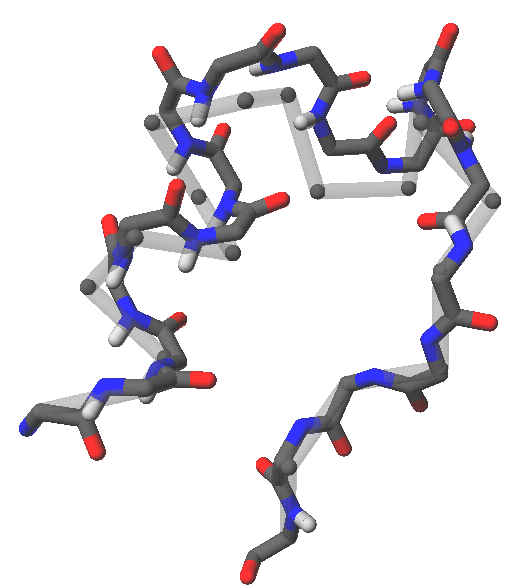
\includegraphics[width=.4\columnwidth]{exampleposter-figures/forside.png}
\vspace{-1.5cm}
\end{figure}
\vspace{1.5cm}

\subsection{Our problem}
Currently, we are only able to predict protein structures at the
$C_\alpha$-trace level.  Our goal with this project is to extend the
\Ca-trace with the remaining atoms to get an all-atom model.  The
difference between the two is shown in Figure
\ref{fig:all-atom_vs_trace}.

\begin{figure}
  \centering
  \vspace{1cm}
  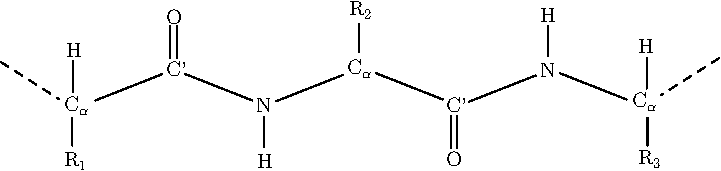
\includegraphics[width=0.65\columnwidth]{exampleposter-figures/amino_connect}  
  \\[1cm]
  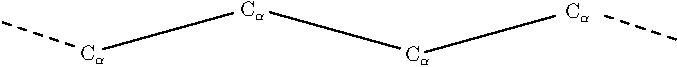
\includegraphics[width=0.65\columnwidth]{exampleposter-figures/Calpha_backbone}
  \caption{\textbf{Top}: All-atom protein backbone, with $R_1$, $R_2$ 
    and $R_3$ representing side-chains. \textbf{Bottom}: $C_{\alpha}$-trace. }
  \label{fig:all-atom_vs_trace}
\end{figure}

\subsection{Our approach}
The folding should be conducted, such that it minimizes the number of
clashes and at the same time minimizes the deviation from the target
$C_\alpha$-trace.

We consider our fitting problem as two somewhat separate problems.
First, we fold the backbone to the \Ca-trace.
Hereafter, the amino acid side-chains are added to the backbone.
\end{multicols}
\end{GridBlock}

\begin{GridBlockFill}{0}{44}{100}

  \begin{multicols}{2}
\begin{minipage}{\linewidth} 
    \begin{multicols}{2}
    \section{Protein Geometry}

    \begin{itemize}
    \item Proteins are built from unbranched chains of amino acids.
    \item All amino acids share
      the same basic structure and a variable side-chain.
    \item The structure of an amino acid can be described by bond lengths,
      bond angles and rotational angles.
    \item The bond lengths and bond angles only displays small variations
      between amino acids (see tables).
    \item Only three different rotational angles occurs along an amino
      acid chain. These are named $\phi$, $\psi$ and $\omega$ and are
      shown on Figure \ref{fig:torsion_angles}.
    \end{itemize} 
   \end{multicols}

\begin{multicols}{2}


\begin{minipage}{\linewidth} 
\centering

  \vspace{7mm}
  \begin{tabular}{lrr}
    \multicolumn{1}{c}{Bond} & \multicolumn{1}{c}{Avg. length} & \multicolumn{1}{c}{Std.dev.} \\ \midrule
    C-O   & 1.2260 Å & 0.0188 Å\\
    CA-C  & 1.5272 Å & 0.0191 Å\\
    N-CA  & 1.4680 Å & 0.0237 Å\\
    C-N   & 1.3234 Å & 0.0215 Å\\
  \end{tabular}
  \vspace{4mm}
  \label{tab:average_bond_lengths}
  \tabcaption{Average bond lengths (in ångstrøm)}
\end{minipage}


\begin{minipage}{\linewidth} 
\centering
  \vspace{7mm}
  \begin{tabular}{lrr}
    \multicolumn{1}{c}{Angle} & \multicolumn{1}{c}{Avg. angle} & \multicolumn{1}{c}{Std.dev.} \\ \midrule 
    H-N-CA & 118.9553$^\circ$ & 1.9979$^\circ$\\
    N-CA-C & 110.6099$^\circ$ & 2.4668$^\circ$\\
    CA-C-N & 116.7804$^\circ$ & 1.7682$^\circ$\\
    C-N-CA & 121.4547$^\circ$ & 1.9946$^\circ$\\
  \end{tabular}
  \vspace{4mm}
  \label{tab:average_bond_angles}
  \tabcaption{Average bond angles}
\end{minipage}

   \end{multicols}
\end{minipage}

\pagebreak

\begin{minipage}{\linewidth} 
\centering% 
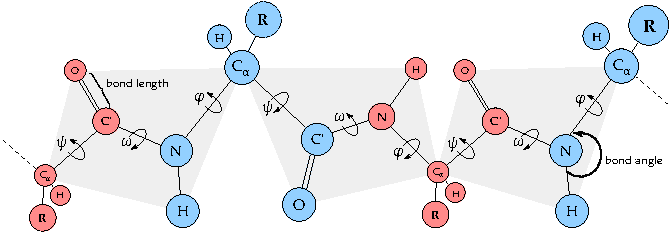
\includegraphics[width=0.90\linewidth, clip=]{exampleposter-figures/protein-torsion-angles.pdf}

\figcaption{Rotational angles in a protein backbone}% 
\label{fig:torsion_angles}
\end{minipage}

\begin{multicols}{2}
  \begin{itemize}
  \item The $\omega$-angle is almost always at $180^{\circ}$, except
    for a few occurrences where it is $0^{\circ}$. To simplify the
    problem, we have assumed that it is always locked at
    $180^{\circ}$.
  \item The $\phi$ and $\psi$ angles are the most variable parts of
    the protein backbone and many models use these as the only
    parameters when performing protein structure prediction.
  \item The $\phi$ and $\psi$ are the only parameters we modify when
    folding the backbone.
  \end{itemize}
\end{multicols}
\end{multicols}



\end{GridBlockFill}

\begin{GridBlock}{0}{72.3}{49}
\begin{multicols}{2}
\section{Backbone folding}

Given a \Ca-trace, we wish to fold the protein backbone (only the
$\phi$ and $\psi$ angles) to match the trace as closely as possible.
The backbone fitting problem can be regarded as an \emph{inverse
  kinematics} problem.

To solve this problem, we have devised an extension to the
\emph{cyclic coordinate descent} (CCD) algorithm:
\begin{itemize}
	\item CCD works by adjusting angles one by one in a greedy manner.
	\item We adjust each angle with the goal of minimizing the mean
    distance between the three forthcoming amino acids $C$ and their
    corresponding \Ca-targets $T$.
	\item The angles are adjusted iteratively in both directions
    interchangably until the deviation has converged.
\end{itemize}

\begin{figure}
  \centering
	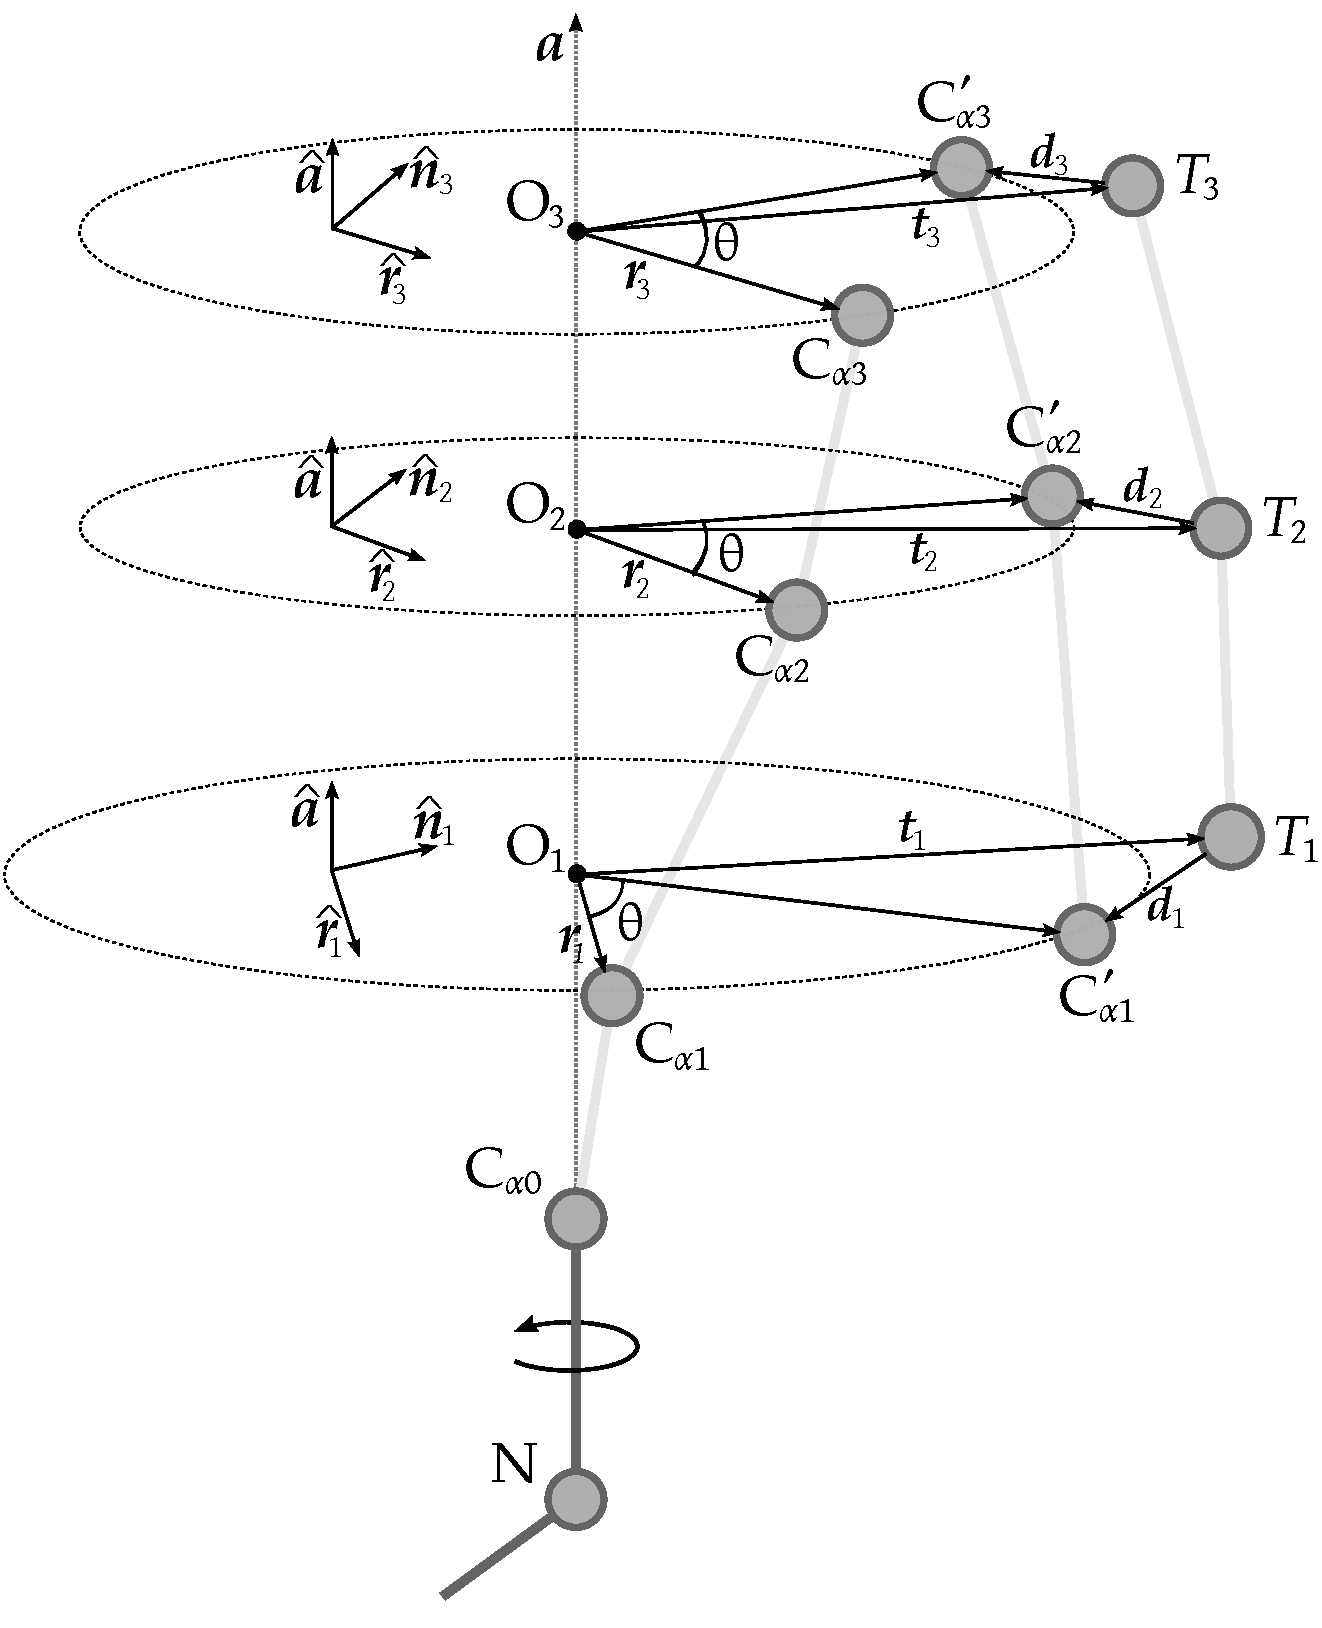
\includegraphics[width=0.85\columnwidth]{exampleposter-figures/ccd}
  \caption{Adjusting an angle according to the \Ca-targets with the CCD algorithm.}
  \label{fig:ccd}
\end{figure}
\end{multicols}
\end{GridBlock}



\begin{GridBlock}{51}{72.3}{49}
\begin{multicols}{2}
\section{Rotamer selection} 
\vspace{-4mm}
\begin{itemize}
\item After the backbone is folded in place and fitted to the
  \Ca-trace, we remain with the problem of adding side chains to each
  amino acid.

\begin{minipage}{\linewidth} 
\centering% 
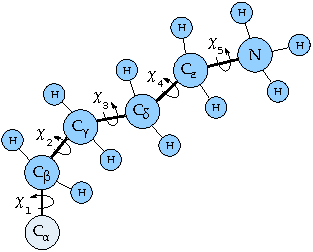
\includegraphics[width=0.90\linewidth, clip=]{exampleposter-figures/lysine.pdf}

\figcaption{$\chi$-angles in Lysine side chain}
\label{fig:lysine}
\end{minipage}
\vspace{1mm}
\item The rotational angles of side chains are named
  $\chi_1$-$\chi_5$, but many amino acids only have one or two of
  these angles.

\item Each side chain tends to have certain configurations of its
  $\chi$-angles. These often occuring configurations are called
  rotamers of the side-chain.

\item There exists rotamer libraries containing these common
  configurations together with their likelihood.

\item We have developed a rotamer search algorithm that minimizes the
  number of occurences, which uses the rotamer-probabilities as a good
  initial guess.
\end{itemize}
\end{multicols}
\end{GridBlock}

\end{document}

